\section{Evaluation}
\label{sectionsimulation}

We carried out a number of experiments in order to validate the radio model. 
All the experiments were carried using LAUNCHXL-CC1350-4 evaluation boards with CC1350 RF microcontrollers 
by Texas Instruments. We used a quiet frequency in the 434~MHz band, for which the boards are designed,
and we used the built-in helix antenna printed on the boards. This antenna is fairly inefficient, resulting
in about 4x to 8x degradation in communication range~\cite{LAUNCHXL-CC1350-4}. We used it because the shorter 
ranges make testing easier
and also because antennas on small wildlife tags also tend to be inefficient due to the tiny ground plane.
The chips that we tested are widely-used in miniature wildlife tags, and they essentially represent a modern
version of the chips that were used on the original Encounternet tags.
% requires more citations.

In all tests we configured the radios for GFSK modulation, 500~kb/s, $\pm 250$~kHz deviation, 1243~kHz receive bandwidth,
and 10~dBm transmit power. We used a Windows program called SmartRF Studio version~7 to drive the boards during
the tests and to log received packets. In all tests one board transmitted one 1.87~packets per second (intevals of
500~ms between packets). Packets consisted of a 4-byte preamble, 4-byte sync workd, a length byte, 30-byte payload 
that includes a sequence number, and a 2-byte checksum. The fast transmission rate reduces power consumption (per byte and
per packet) and leads to short communication ranges, which are consistent with the goal of registering close encounters.

In a preliminary test, we configured one board to transmit packets, one board to receive them, and a third to transmit a 
CW carrier at the same frequency. The three boards were at distances of 0.4~m from each other. When the CW transmitter
was off, virtually all packets were received correctly. When the CW transmitter was on, virtually no packets were received.
This verifies that interference indeed blocks the receiver and may prevent packets from being received.
% It would have been good to transmit two packets simulteneously but there is no easy way to synchronize the boards.

\begin{figure}[h]
    \centering
    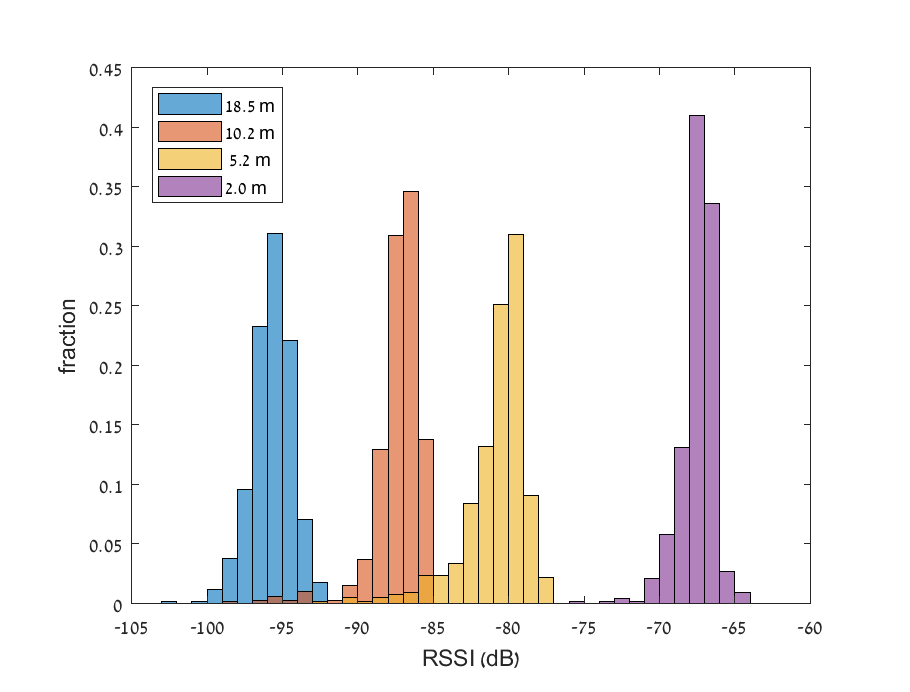
\includegraphics[width=3.5in]{experiments/rssiHistograms.eps}
    \caption{Histograms of the RSSI of received packets at different distances between the transmitter and the receiver.}
    \label{fig:rssiHistograms}
\end{figure}

\begin{figure}[h]
    \centering
    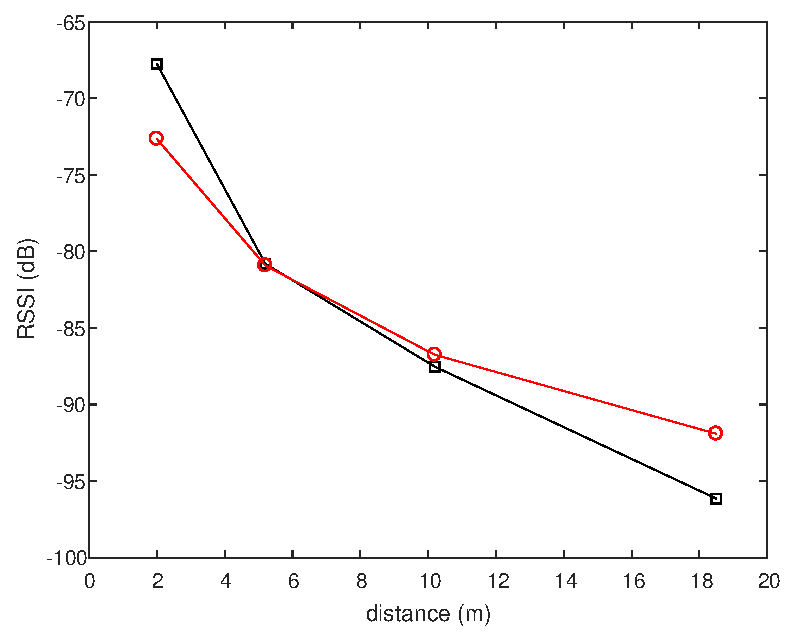
\includegraphics[width=3.5in]{experiments/rssiDistance.eps}
    \caption{Mean RSSI (after removal of outliers) at different distances, in black. The red curve is a least-square
    fitting of the data to a 6~dB attenuation when the distance doubles.}
    \label{fig:rssiDistance}
\end{figure}

In the main test, we placed the transmitter board at a fixed position, about 1.4~m above ground, and measured receive
performance at various distances between 2 and 78~m in an outdoor area with some human activity (but not much). We 
maintained each test position for at least 5 minutes.
The receiver board was also placed about 1.4~m above ground. In all the tests shown in graphs the transmit
and receive antennas were pointed at each other. We also performed a few tests with the receive antenna rotated 90~degrees;
RSSI values were about 1--2~dB lower but the overall results were similar; this is consistent with the characterization
of the antenna, which indicates that it is fairly onmidirectional~\cite{LAUNCHXL-CC1350-4}.
The main results are shown in Figure~\ref{fig:rssiHistograms}.
At each distance we measured the fraction of correctly-received packets and the RSSI of each packet. At the four
distances reported in the figure, virtually all transmitted packets were received correctly. We can see a clear
statistical correlation between distance and RSSI. Figure~\ref{fig:rssiDistance} shows that the RSSI values
roughly follow the theoretical rule that stipulates a 6~dB attenuation when the distance doubles. The means
shown in this figure are of the center 50\% of the packets; the extreme 50\% were filtered to remove outliers.

We also tested performance at distances of 53~m and 78~m. At these distances, results were inconsistent. In one test
at 78~m, 84\% of the packets with mean RSSI of -98~dB. But in another test two hours later, only 2\% of the packets
were correctly received. At 53~m, no packets were received correctly for over 5 minutes. This location was in a depression,
about 3~m lower than both the transmitter and from the 78~m position; this may have contributed to the worse performance.
The main conclusion from these long-distance experiments (long given the bit rate) is that packets can sometimes be received
at fairly long distances and with RSSI values that typically characterize much shorter distances. 

However, the results also indicate that by dropping packets with low RSSI, say below -90~dB for these settings, we can
effectively limit the communication range to 20~m or so.
